
%(BEGIN_QUESTION)
% Copyright 2006, Tony R. Kuphaldt, released under the Creative Commons Attribution License (v 1.0)
% This means you may do almost anything with this work of mine, so long as you give me proper credit

Given the choice between these two wiring options (keeping the transmitter close to the process versus far away), which is best, and why?

$$\includegraphics[width=15.5cm]{i00392x01.eps}$$

$$\includegraphics[width=15.5cm]{i00392x02.eps}$$

\vskip 20pt \vbox{\hrule \hbox{\strut \vrule{} {\bf Suggestions for Socratic discussion} \vrule} \hrule}

\begin{itemize}
\item{} If the longer wire in each case were {\it shielded}, how should we ground the shield for best results?
\item{} How could we use a {\it loop calibrator} to ``trick'' the indicator into thinking the thermocouple was at some particular temperature when in fact it was not?
\end{itemize}

\underbar{file i00392}
%(END_QUESTION)





%(BEGIN_ANSWER)

Thermocouple signals are very small, and the input impedance of a thermocouple transmitter is typically large, making it susceptible to electrical interference.  Given this fact, it is better to minimize the length of the noise-gathering signal path (the thermocouple wire).  Also, thermocouple wire (even extension-grade wire) is more expensive than similar-gauge copper, which makes long lengths of copper cheaper than long lengths of thermocouple wire.

%(END_ANSWER)





%(BEGIN_NOTES)









\vskip 20pt \vbox{\hrule \hbox{\strut \vrule{} {\bf Virtual Troubleshooting} \vrule} \hrule}

This question is a good candidate for a ``Virtual Troubleshooting'' exercise.  Presenting the diagram to students, you first imagine in your own mind a particular fault in the system.  Then, you present one or more symptoms of that fault (something noticeable by an operator or other user of the system).  Students then propose various diagnostic tests to perform on this system to identify the nature and location of the fault, as though they were technicians trying to troubleshoot the problem.  Your job is to tell them what the result(s) would be for each of the proposed diagnostic tests, documenting those results where all the students can see.

During and after the exercise, it is good to ask students follow-up questions such as:

\begin{itemize}
\item{} What does the result of the last diagnostic test tell you about the fault?
\item{} Suppose the results of the last diagnostic test were different.  What then would that result tell you about the fault?
\item{} Is the last diagnostic test the best one we could do?
\item{} What would be the ideal order of tests, to diagnose the problem in as few steps as possible?
\end{itemize}

%INDEX% Measurement, temperature: thermocouple

%(END_NOTES)


